% Member 1 (T1). Figure: python -m project4.experiments.t1_expected_loss
\section{Decision theory with a reject option}
\label{sec:decision}

This section answers Task~1. We fix the loss matrix, derive the action that minimises the posterior
expected loss for any loss matrix, and then obtain explicit probability thresholds for our spam filter.
Throughout, $\post = \post(x) = \Prob(y=1\mid x)$ is the posterior probability that email $x$ is spam.

\subsection{Loss matrix and the inspection assumption}
\label{sec:loss-matrix}

The filter takes one of three actions: deliver ($a=0$), send to the spam folder ($a=1$), or hold for
human inspection ($a=r$). Table~\ref{tab:loss} gives the loss $L(a,y)$ of each action for each true label.

\begin{table}[ht]
\centering
\begin{tabular}{lcc}
\toprule
Action $\backslash$ true label & $y=0$ (real email) & $y=1$ (spam) \\
\midrule
$a=0$ deliver        & $0$     & $\cfn$ \\
$a=1$ spam folder    & $\cfp$  & $0$ \\
$a=r$ inspect        & $\ci$   & $\ci$ \\
\bottomrule
\end{tabular}
\caption{Loss matrix $L(a,y)$. Default values: $\cfp=10$, $\cfn=1$, $\ci=0.3$; the experiments sweep $\cfp/\cfn$ and $\ci$.}
\label{tab:loss}
\end{table}

\paragraph{Why these numbers.}
\begin{itemize}[itemsep=1pt,topsep=2pt]
  \item \emph{Correct decisions cost $0$.} Only relative losses matter, so we measure every loss against
        the outcome of a perfect filter.
  \item \emph{$\cfp=10$.} A real email in the spam folder is usually never seen: the reader may miss a
        reply, an invoice or a job offer. This is the worst outcome.
  \item \emph{$\cfn=1$.} A spam in the inbox costs a few seconds to recognise and delete. We use it as
        the unit of loss.
  \item \emph{$\ci=0.3$.} Held emails go to a review queue that a person scans in batches. Checking one
        is cheaper than dealing with a spam in the inbox, but not free. This value is a placeholder:
        Section~\ref{sec:accuracy-cost} varies $\ci$ over its whole range.
\end{itemize}
Only the ratios $\cfp:\cfn:\ci$ affect the decisions, because multiplying every loss by a constant
does not change which action is cheapest.

\paragraph{Inspection assumption.}
Inspection costs $\ci$ whatever the true label, and the inspector always finds the true label and
routes the email correctly. So no further loss follows an inspection, and the inspect row of
Table~\ref{tab:loss} is constant.

\paragraph{Variant: imperfect inspection.}
Suppose instead that the inspector sends a real email to spam with probability $\varepsilon_0$ and
delivers a spam with probability $\varepsilon_1$. The inspect row becomes
$L(r,0)=\ci+\varepsilon_0\cfp$ and $L(r,1)=\ci+\varepsilon_1\cfn$, which is no longer constant.
The general result below (Proposition~\ref{prop:bayes}) still applies, and repeating the derivation of
Section~\ref{sec:thresholds} gives the thresholds
\[
  \thz' = \frac{\ci+\varepsilon_0\cfp}{(1-\varepsilon_1)\cfn+\varepsilon_0\cfp},
  \qquad
  \tho' = \frac{(1-\varepsilon_0)\cfp-\ci}{(1-\varepsilon_0)\cfp+\varepsilon_1\cfn}.
\]
For $\varepsilon_0=\varepsilon_1=0$ these reduce to \eqref{eq:thresholds} below. Whenever the band
exists ($\ci<\cfn$ is then automatic), $\thz'\ge\thz$ and $\tho'\le\tho$: an unreliable inspector is
used for fewer emails. We keep the perfect-inspection assumption in the rest of the report.

\subsection{The Bayes action for a general loss matrix}
\label{sec:bayes-action}

Let $L(a,y)$ be any loss matrix with a finite set of actions $\mathcal A$ and labels $y\in\{0,1\}$.
The \emph{posterior expected loss} (conditional risk) of action $a$ for email $x$ is
\begin{equation}
  R(a\mid x) = \sum_{y\in\{0,1\}} L(a,y)\,\Prob(y\mid x) = (1-\post)\,L(a,0) + \post\,L(a,1).
  \label{eq:cond-risk}
\end{equation}

\begin{proposition}[Bayes action]\label{prop:bayes}
Among all decision rules $\delta:x\mapsto\delta(x)\in\mathcal A$, the expected loss
$\E\big[L(\delta(x),y)\big]$ is minimised by
\[
  \delta^\ast(x) = \arg\min_{a\in\mathcal A} R(a\mid x).
\]
\end{proposition}

Two consequences follow from \eqref{eq:cond-risk}. First, $R(a\mid x)$ depends on $x$ only through
$\post(x)$, so the Bayes action is a function of the posterior alone. Second, each $R(a\mid x)$ is an
affine function of $\post$, so the minimum over actions is the lower envelope of straight lines.
That envelope is concave and piecewise linear, and every action is optimal on a single interval of
$\post$ (possibly empty). Hence the Bayes rule always has the form ``compare $\post$ with thresholds''.
The rest of this section finds those thresholds.

\subsection{Explicit thresholds}
\label{sec:thresholds}

With the loss matrix of Table~\ref{tab:loss}, \eqref{eq:cond-risk} gives
\begin{equation}
  R(0\mid x) = \cfn\,\post, \qquad R(1\mid x) = \cfp\,(1-\post), \qquad R(r\mid x) = \ci .
  \label{eq:three-risks}
\end{equation}
Comparing the actions two at a time:
\begin{align*}
  \text{deliver vs.\ spam folder:}\quad & \cfn\post \le \cfp(1-\post) &&\iff \post \le \frac{\cfp}{\cfp+\cfn} = \tstar, \\
  \text{deliver vs.\ inspect:}\quad     & \cfn\post \le \ci           &&\iff \post \le \frac{\ci}{\cfn} = \thz, \\
  \text{spam folder vs.\ inspect:}\quad & \cfp(1-\post) \le \ci       &&\iff \post \ge 1-\frac{\ci}{\cfp} = \tho .
\end{align*}

\begin{proposition}[Reject thresholds]\label{prop:band}
Let $\cstar = \dfrac{\cfp\,\cfn}{\cfp+\cfn}$.
\begin{enumerate}[label=(\alph*),itemsep=1pt,topsep=2pt]
  \item If $\ci<\cstar$, then $\thz<\tstar<\tho$ and the Bayes action is
        \begin{equation}
          \delta^\ast(x) =
          \begin{cases}
            \text{deliver}     & \text{if } \post \le \thz = \ci/\cfn, \\
            \text{inspect}     & \text{if } \thz < \post < \tho, \\
            \text{spam folder} & \text{if } \post \ge \tho = 1-\ci/\cfp .
          \end{cases}
          \label{eq:thresholds}
        \end{equation}
  \item If $\ci\ge\cstar$, inspection is never strictly better than the best automatic action, and the
        Bayes action is the single-threshold rule: spam folder iff $\post\ge\tstar$, deliver otherwise.
\end{enumerate}
\end{proposition}

The inspect band $(\thz,\tho)$ is non-empty exactly when
\[
  \thz<\tho \iff \frac{\ci}{\cfn}+\frac{\ci}{\cfp}<1 \iff \ci<\cstar .
\]
$\cstar$ is half the harmonic mean of the two error costs, so it is always below $\min\{\cfp,\cfn\}$:
inspection must be cheaper than the cheaper error to be worth using. At the boundary values
$\post=\thz$ and $\post=\tho$ two actions have equal risk; the code (\texttt{decision.bayes\_action})
breaks these ties towards the automatic action.

\paragraph{Our default values.}
With $\cfp=10$, $\cfn=1$ we get $\tstar=\cstar=10/11\approx0.909$. With $\ci=0.3$ the band exists and
\[
  \thz = 0.3, \qquad \tho = 0.97 .
\]
The rule is strongly asymmetric. An email goes to the spam folder only if the model is at least $97\%$
sure it is spam, because a wrong spam-folder decision costs ten times as much as a wrong delivery. The
lower threshold $\thz=\ci/\cfn$ depends only on the cost of delivering spam, and the upper threshold
$\tho=1-\ci/\cfp$ only on the cost of losing a real email. Figure~\ref{fig:t1-loss} shows the three
lines of \eqref{eq:three-risks}, their lower envelope and the resulting decision regions.

\begin{figure}[ht]
\centering
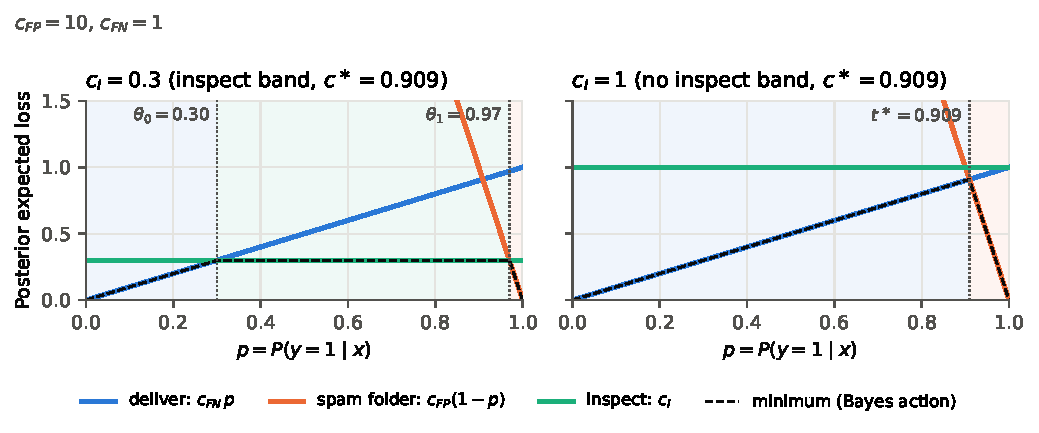
\includegraphics[width=\linewidth]{../project4/figures/t1_expected_loss.pdf}
\caption{Posterior expected loss of each action against $\post$ for $\cfp=10$, $\cfn=1$. Shading shows
where each action is optimal. Left: $\ci=0.3<\cstar$, so the inspect band is $(0.3,\,0.97)$.
Right: $\ci=1>\cstar$, so the inspect line never reaches the envelope and the rule is the single
threshold $\tstar=10/11$. Generated by \texttt{experiments/t1\_expected\_loss.py}.}
\label{fig:t1-loss}
\end{figure}

\subsection{Check: equal error costs give the classic reject rule}
\label{sec:chow}

If both errors cost the same, $\cfp=\cfn=c$, then $\thz=\ci/c$ and $\tho=1-\ci/c$, and we inspect iff
\[
  \frac{\ci}{c}<\post<1-\frac{\ci}{c}
  \iff \max\{\post,\,1-\post\} < 1-\frac{\ci}{c}
  \iff \max_{k\in\{0,1\}}\Prob(k\mid x) < 1-\frac{\ci}{c} .
\]
This is Chow's reject rule~\cite{chow1970,bishop2006}: inspect when even the most likely label is not
likely enough. Here $\cstar=c/2$, so rejection is used only if inspecting costs less than half an error.
For $c=1$ (0--1 loss) and $\ci\to\infty$ it reduces to the accuracy-based rule ``predict the more
probable label'', i.e.\ threshold $1/2$. That rule is optimal only when $\cfp=\cfn$; with our costs
the threshold is $\tstar=10/11$, not $1/2$.

\begin{assumptions}
Losses depend only on the action and the true label and add up over emails; correct decisions cost $0$;
$\cfp,\cfn>0$ and $\ci\ge0$ are constants; the inspector is always right; and $\post$ is the true
posterior. A model's estimate $\hat\post$ gives the Bayes action only if it is calibrated
(Section~\ref{sec:calibration}).
\end{assumptions}

\noindent The code implements \eqref{eq:thresholds} in \texttt{decision.bayes\_action}. A unit test
compares it with a brute-force minimisation of \eqref{eq:cond-risk} on $10{,}000$ random posteriors and
loss matrices (see the experimental setup in Section~1).
